\chapter{Interrupts}
In dit hoofdstuk worden interrupts en het interruptmechanisme van de ATmega32
behandeld.

\section{Polling}
De ATmega32 kan met behulp van een wachtlus reageren op signalen van
externe bronnen. De externe bronnen kunnen zo aan de processor aangeven
dat er bijvoorbeeld data beschikbaar is en dat afhandeling is gewenst.
Dat werkt als volgt. De ATmega32 leest een byte in van een van de
I/O-poorten. Vervolgens wordt de bit die getest moet worden met behulp
van een bitmasker gefilterd. Is de geteste bit niet actief, dan wordt
opnieuw een byte ingelezen en begint het testen opnieuw. Is de geteste
bit wel actief, dan wordt de wachtlus verlaten en wordt de rest van het
programma uitgevoerd. 
Deze methode wordt \textsl{polling} genoemd. In het vakgebied van de
Operating Systems wordt dit \textsl{busy waiting} genoemd.

In listing~\ref{cod:intpolling} is een voorbeeld van zo'n wachtlus te zien.
Eerst wordt de status van de pinnen van Port A ingelezen door middel van
een \lstinline|in|-instructie. De \lstinline|andi|-instructie zorgt ervoor
dat de minst significante bit wordt gefilterd; de overige bits worden op~0
gezet. De \lstinline|andi|-instructie past ook de Z-vlag aan. Als blijkt
dat de minst significante bit een~0 is dan wordt de Z-vlag op~1 gezet,
anders wordt de Z-vlag op~0 gezet (merk op dat de overige bits op~0 gezet
zijn). Als blijkt dat de minst significante bit een~0 is, dan zorgt de
\lstinline|breq|-instructie ervoor dat weer naar het begin van de wachtlus
wordt gesprongen. Is de minst significante bit een~1, dan wordt de lus
verlaten en wordt de eerstvolgende instructie uitgevoerd. 

\begin{lstlisting}[language=AVRassembler,caption=Polling.,label=cod:intpolling]
loop:	in   r16,PINA   ; read in pins Port A
		andi r16,0x01   ; filter LSB, Z-flag = 1 if bit = 0
		breq loop       ; again if bit is 0
\end{lstlisting}

Deze manier van detectie werkt eenvoudig en snel. Het programma (de wachtlus)
is eenvoudig en er zijn slechts enkele klokpulsen nodig om de status van een
extern signaal te bepalen. Het nadeel is natuurlijk dat de processor niets
anders kan doen.


\section{Interrupts}
Slimmer is om de hardware aan de processor door te laten geven dat de status
van een signaal is veranderd, zodat de processor direct actie kan ondernemen.
Het lopende programma wordt dan \textsl{geïnterrumpeerd} (onderbroken).
Dit wordt een \textsl{interrupt} genoemd. Een aanvraag voor een onderbreking
(het signaal) wordt een \textsl{interrupt request} (IRQ) genoemd.

Nadat een interrupt request door de processor is herkend, wordt het lopende
programma onderbroken (de huidige instructie wordt afgemaakt) en wordt een
\textsl{interrupt service routine} (ISR) uitgevoerd. De ISR handelt dan de
interrupt verder af. Daarna gaat de processor verder waar het gebleven was.

We beelden dit uit in figuur~\ref{fig:intsimpleinterruptdispatch}. Hierin
stelt \textsf{H} de uitvoer van het lopende programma voor. Op een gegeven
moment wordt er een interrupt geregistreerd door de processor. Het lopende
programma wordt verlaten en de processor gaat de ISR uitvoeren. Aan het einde
van de ISR wordt teruggekeerd naar het lopende programma \textsf{H}.

\begin{figure}[!ht]
\centering
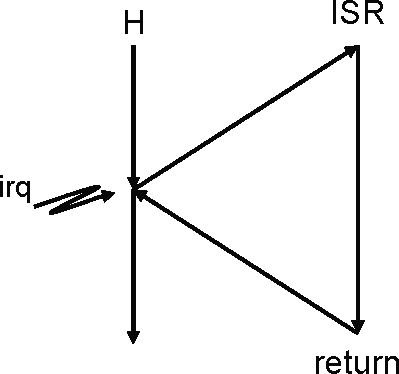
\includegraphics[scale=\figscale]{images/intsimpleinterruptdispatch}
\caption{Eenvoudige voorstelling van een interruptafhandeling.}
\label{fig:intsimpleinterruptdispatch}
\end{figure}

ISR's lijken veel op gewone subroutines, maar er zijn verschillen:

\begin{itemize}
\item Een ISR wordt gestart door een interrupt, niet door een
instructie\footnote{Er zijn processoren die instructies hebben die
software-interrupts genereren, zoals de Intel x86-familie.}.

\item Direct nadat de interrupt is herkend, wordt de Global Interrupt Enable
vlag (de I-vlag) in het Status Register op 0 gezet. Dit zorgt ervoor dat de
ISR niet kan worden onderbroken door een (nieuwe) interruptaanvraag.

\item Voor terugkeer moet de instructie \lstinline|RETI| (Return From
Interrupt) gebruikt worden. Deze instructie zet de Global Interrupt Enable
vlag weer aan.
\end{itemize}

Interrupts en subroutines hebben wel \'e\'en overeenkomst: in beide gevallen
wordt de program counter (PC) op de stack gezet. Dit wordt uitgebeeld in
figuur~\ref{fig:intinterruptdispatchwithstackandiflag}. Omdat het
terugkeeradres op de stack wordt gezet, moet de stack pointer (SP) worden
ge\"initialiseerd v\'o\'ordat de interrupts mogen worden afgehandeld. Dat
betekent dat direct naar het starten van het lopende programma, bijvoorbeeld
na een reset, de interrupts nog niet mogen worden afgehandeld omdat de
stack pointer nog niet is ge\"initialiseerd.

\begin{figure}[!ht]
\centering
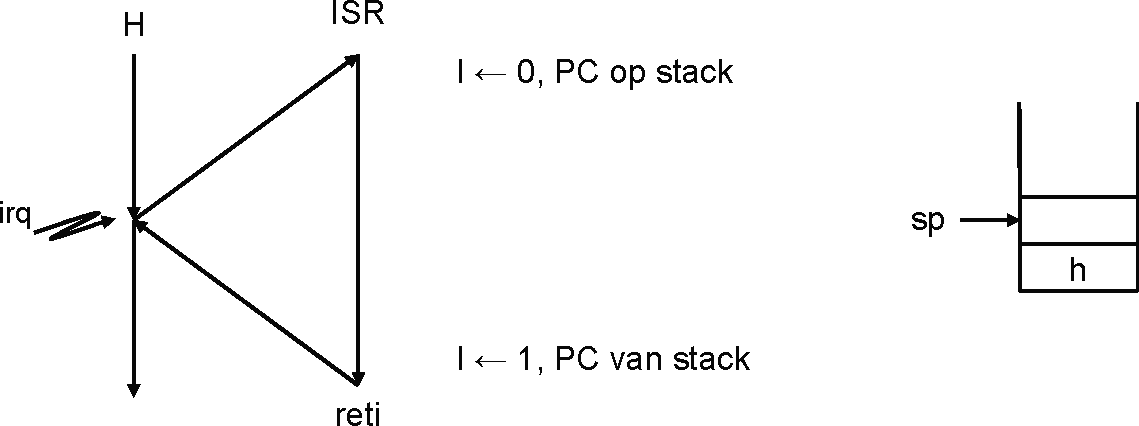
\includegraphics[scale=\figscale]{images/intinterruptdispatchwithstackandiflag}
\caption{Interruptafhandeling: de Program Counter wordt op de stack gezet.}
\label{fig:intinterruptdispatchwithstackandiflag}
\end{figure}

Twee instructies be\"invloeden direct de I-flag:

\qquad \lstinline|sei| - set Global Interrupt Enable flag, interrupts worden afgehandeld.

\qquad\lstinline|cli| - clear Global Interrupt Enable flag, interrupts worden geblokkeerd.

De I-vlag is gepositioneerd op bit 7 van het Status Register (SREG). Zie
figuur~\ref{fig:intsregregisterlayout}.

%%%% SREG
\begin{figure}[!ht]
\renewcommand\arraystretch{1.4}
%\footnotesize
\scriptsize
\centering
\begin{tabu} to 0.9\textwidth {X[,c,]X[,c,]X[,c,]X[,c,]X[,c,]X[,c,]X[,c,]X[,c,]}
7 & 6 & 5 & 4 & 3 & 2 & 1 & 0 \\
\hline
\multicolumn{1}{|c}{I} & \multicolumn{1}{|c}{T} & \multicolumn{1}{|c}{H} & \multicolumn{1}{|c}{S} & \multicolumn{1}{|c}{V} & \multicolumn{1}{|c}{N} & \multicolumn{1}{|c}{Z} & \multicolumn{1}{|c|}{C} \\ \hline
R/W & R/W & R/W & R/W & R/W & R/W & R/W & R/W \\
0 & 0 & 0 & 0 & 0 & 0 & 0 & 0 \\
\end{tabu}
\caption{Status Register SREG.}
\label{fig:intsregregisterlayout}
\end{figure}
%%%% SREG

Pas na het initialiseren van de stack pointer mag de instructie
\lstinline|sei| gegeven worden.


\section{Interruptbronnen}
De ATmega32 kent veel interruptbronnen. Zo kan de ATmega32 reageren op
drie externe interrupts: INT0, INT1 en INT2. Verder kan de analoog-digitaal
converter (ADC) een interrupt geven als de conversie klaar is. De seri\"ele
interface (USART) kent naast een interrupt wanneer een karakter is ontvangen
ook een interrupt voor wanneer een karakter is verzonden. De nog te bespreken
timer/counters (zie hoofdstuk~\ref{cha:timercounters}) kunnen een interrupt
afgeven wanneer een timer/counter ``over de kop'' gaat, dus wanneer een
timer/counter van de hoogste stand naar de laagste stand gaat. Verder zijn
er nog interrupts mogelijk van de EEPROM, de TWI- en de SPI-interface.

Al deze interruptbronnen hebben een eigen interrupt-enable-bit. Om een
interrupt van een bron ook daadwerkelijk te laten plaatsvinden, moet deze
bit geactiveerd zijn (logisch~1) \'en de I-vlag moet logisch 1 zijn.

De ATmega32 heeft geen \textsl{software interrupts}. Dat zijn
software-instructies die interrupts genereren. Deze zijn wel na te bootsen
met INT0, INT1 en INT2.


\section{De Interrupt Vector Table}
We hebben nu besproken hoe het verwerken van een interrupt wordt uitgevoerd.
Maar nu rijst de vraag: waar moet de ISR beginnen? We zouden hiervoor een
vast adres in de Flash-ROM kunnen kiezen, bijvoorbeeld adres 0x1000.
Vervolgens reserveren we 512 bytes voor de ISR. De volgende ISR begint dan
op adres 0x1200. Hoewel dit natuurlijk te realiseren is, kleven hier wel
wat bezwaren aan. Ten eerste moet de ISR altijd op adres 0x1000 beginnen.
Ten tweede kan de ISR niet groter zijn dan 512 bytes. Als de ISR korter is
dan 512 bytes, dan gebruiken we een gedeelte van de Flash-ROM niet (bedenk
dat de volgende ISR op adres 0x1200 begint). Ten derde moet de Flash-ROM
minimaal 4608 (= 0x1200) bytes groot zijn. We zien nu dat een vast adres
en een vaste lengte voor een ISR niet flexibel is.

We kunnen deze drie problemen oplossen door gebruik te maken van een
\textsl{Interrupt Vector Table}.






\begin{figure}[!ht]
\centering
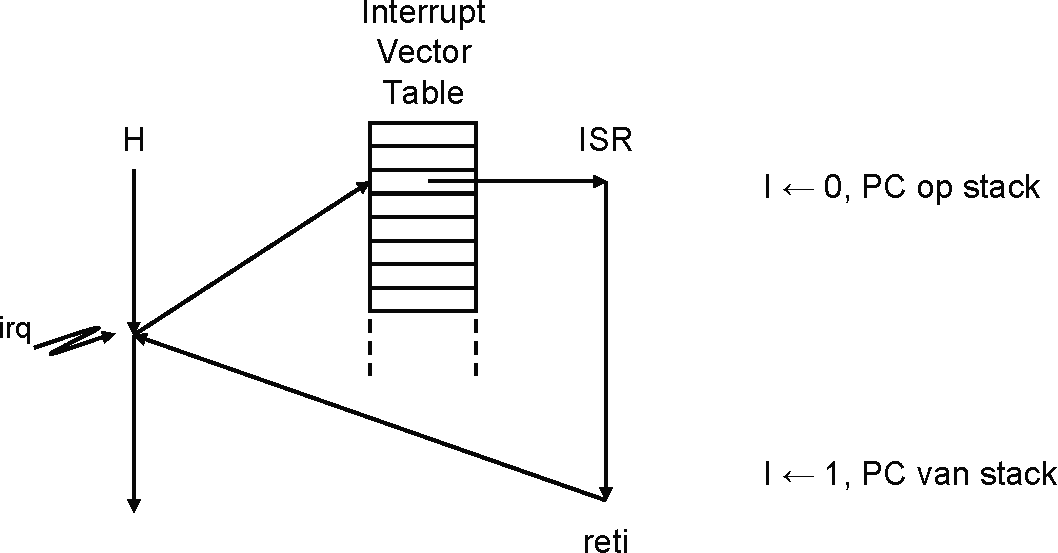
\includegraphics[scale=\figscale]{images/intinterruptdispatchwithvectortable}
\caption{Interruptafhandeling: gebruik van de Interrupt Vector Table.}
\label{fig:intinterruptdispatchwithvectortable}
\end{figure}



\section{Stappen in de interruptverwerking}
Als een interruptsignaal bij de processor binnenkomt, worden de volgende
stappen genomen:
\begin{enumerate}
\item De processor maakt de instructie af die op dat moment wordt uitgevoerd.
      Dit is een instructie in het programma.
\item De processor slaat het adres van de volgende instructie op de stack op.
      Dit adres staat in de program counter. De Global Interrupt Enable vlag
      wordt op 0 gezet.
\item De processor springt naar de \textsl{interrupt vector}. Dit is een vaste
      geheugenlocatie in de Flash-ROM.
\item Vanuit de interrupt vector wordt gesprongen naar naar het adres van de
      daadwerkelijke interrupt service routine (ISR).
\item Bij terugkeer uit de ISR wordt de program counter geladen met de adres
      dat op de stack gezet was. De Global Interrupt Enable vlag wordt op 1
      gezet.
\item De processor vervolgt het uitvoeren van het programma. Er wordt altijd
      \'e\'en instructie uitgevoerd voordat een eventuele nieuwe interrupt
      wordt verwerkt.
\end{enumerate}

\begin{table}[!ht]
\centering
\caption{Interrupt vectortabel voor de ATmeag32(A).}
\setlength{\tabcolsep}{8pt}
\begin{tabu}{ccll}
\toprule
vector \# & ROM-adres & Bron          & Omschrijving \\ \midrule
 1        & 0x000     & RESET         & Reset vector \\
 2        & 0x002     & INT0          & External Interrupt request 0 \\
 3        & 0x004     & INT1          & External Interrupt request 1 \\
 4        & 0x006     & INT2          & External Interrupt request 2 \\
 5        & 0x008     & TIMER2\_COMP  & Timer/Counter2 Compare Match \\
 6        & 0x00A     & TIMER2\_OVF   & Timer/Counter2 Overflow \\
 7        & 0x00C     & TIMER1\_CAPT  & Timer/Counter1 Capture Event \\
 8        & 0x00E     & TIMER1\_COMPA & Timer/Counter1 Compare Match A \\
 9        & 0x010     & TIMER1\_COMPB & Timer/Counter1 Compare Match B \\
10        & 0x012     & TIMER1\_OVF   & Timer/Counter1 Overflow \\
11        & 0x014     & TIMER0\_COMP  & Timer/Counter0 Compare Match \\
12        & 0x016     & TIMER0\_OVF   & Timer/Counter0 Overflow \\
13        & 0x018     & SPI, STC      & Serial Transfer Complete \\
14        & 0x01A     & USART, RXC    & USART, Rx Complete \\
15        & 0x01C     & USART, UDRE   & USART Data Register Empty \\
16        & 0x01E     & USART, TXC    & USART, Tx Complete \\
17        & 0x020     & ADC           & ADC Conversion Complete \\
18        & 0x022     & EE\_RDY       & EEPROM Ready \\
19        & 0x024     & ANA\_COMP     & Analog Comparator \\
20        & 0x026     & TWI           & Two-wire Serial Interface \\
21        & 0x028     & SPM\_RDY      & Store Program Memory Ready \\
\bottomrule
\end{tabu}
Noot: het ROM-adres is in words.
\end{table}

\section{Interruptresponstijd}
De responstijd voor alle ingeschakelde interrupts van de ATmega32 is minimaal vier klokcycli.
Tijdens deze vier klokcyclusperiode wordt de program counter op de stack geplaatst (twee bytes)
en wordt de program counter geladen met het vectoradres van de interrupt.
Na vier klokcycli wordt gesprongen naar het vectoradres van de interrupt die wordt gehonoreerd.
De instructie op de vector is normaal gesproken een sprong naar de interruptroutine en deze
sprong duurt drie klokcycli.

Als een interrupt optreedt tijdens de uitvoering van een instructie met meerdere cycli dan
wordt deze instructie voltooid voordat de interrupt wordt gehonoreerd. Staat de ATmega32 in
slaapstand dan wordt de responstijd met vier klokcycli verhoogd. Deze verhoging komt bovenop
de opstarttijd van de geselecteerde slaapmodus.

Een terugkeer (return) uit een interruptroutine duurt vier klokcycli. Tijdens deze vier
klokcycli wordt de program counter van de stack gehaald (twee bytes) en wordt de stack
pointer met twee verhoogd. Tevens word de I-bit in het statusregister op 1 gezet.

\section{Context switch}

\begin{lstlisting}[language=AVRassembler,caption=Opslaan van de vlaggen.,label=cod:contextswich]
ISR:	push r16		; push R16
		in   r16,SREG	; SREG in I/O memory ...
		push r16		; ... so push flags via R16

		pop  r16		; pop flags via R16
		out  SREG,r16
		pop  r16		; pop R16
		reti			; return
\end{lstlisting}

\section{Externe interrupts}
De General Interrupt Control Register (GICR) heeft drie bits waarmee de INT’s kunnen worden geactiveerd.

Een logische 1 in het betreffende bit activeert de INT.

De I-flag moet 1 zijn om interrupt ook daadwerkelijk te herkennen.


%%%% GICR
\begin{figure}[!ht]
\renewcommand\arraystretch{1.4}
%\footnotesize
\scriptsize
\centering
\begin{tabu} to 0.9\textwidth {X[,c,]X[,c,]X[,c,]X[,c,]X[,c,]X[,c,]X[,c,]X[,c,]}
7 & 6 & 5 & 4 & 3 & 2 & 1 & 0 \\
\hline
\multicolumn{1}{|c}{INT0} & \multicolumn{1}{|c}{INT1} & \multicolumn{1}{|c}{INT2} & \multicolumn{1}{|c}{\cellcolor{lightgrey} $-$} & \multicolumn{1}{|c}{\cellcolor{lightgrey} $-$} & \multicolumn{1}{|c}{\cellcolor{lightgrey} $-$} & \multicolumn{1}{|c}{\cellcolor{lightgrey} IVSEL} & \multicolumn{1}{|c|}{\cellcolor{lightgrey} IVCE} \\ \hline
R/W & R/W & R/W & R/W & R/W & R/W & R/W & R/W \\
0 & 0 & 0 & 0 & 0 & 0 & 0 & 0 \\
\end{tabu}
\caption{GICR register}
\label{fig:intgicr}
\end{figure}
%%%% GICR
